%% main_report50.tex
%% SAMBP TR-50/2026: Wide-Area Protection Coordinator (WAPC)
%%
%% pdflatex main_report50.tex

\documentclass[11pt,a4paper]{article}

\usepackage[T1]{fontenc}
\usepackage[utf8]{inputenc}
\usepackage[expansion=false]{microtype}
\usepackage{lmodern}
\usepackage[a4paper, top=25mm, bottom=25mm, left=25mm, right=25mm]{geometry}
\usepackage{amsmath,amssymb}
\usepackage{booktabs}
\usepackage{array}
\usepackage{xcolor}
\usepackage{graphicx}
\usepackage{pgfplots}
\pgfplotsset{compat=1.18}
\usepackage{tikz}
\usetikzlibrary{arrows.meta,shapes.geometric,positioning,fit,calc}
\usepackage{hyperref}
\usepackage[numbers,sort&compress]{natbib}

\definecolor{sambpblue}{RGB}{0,70,140}

\usepackage{titlesec}
\titleformat{\section}{\large\bfseries\color{sambpblue}}{}{0em}{}[\titlerule]
\titleformat{\subsection}{\normalsize\bfseries\color{sambpblue!80}}{}{0em}{}

\usepackage{fancyhdr}
\pagestyle{fancy}
\fancyhf{}
\rhead{\small\color{gray} SAMBP TR-50/2026}
\lhead{\small\color{gray} Wide-Area Protection Coordinator}
\cfoot{\small\thepage}

\begin{document}

\begin{center}
  {\LARGE\bfseries\color{sambpblue} SAMBP Technical Report TR-50/2026}\\[6pt]
  {\large Wide-Area Protection Coordinator (WAPC)}\\[10pt]
  {\normalsize PhD Thesis Supporting Report \quad|\quad 2026}
\end{center}

\vspace{2pt}\hrule\vspace{8pt}

\begin{abstract}
\noindent
This report develops the Wide-Area Protection Coordinator (WAPC), a
centralised decision engine that aggregates IED relay reports and PMU
synchrophasor data across a 10-bus IBR test network to deliver four
capabilities unavailable to individual relays: (i) network-wide fault
localisation, (ii) N-1 security verification before tripping, (iii)
PINN ML advisory integration, and (iv) coordinated GOOSE messaging.
Study B demonstrates 94.5\% correct-line fault localisation at standard
IEC\,Class\,P1 PMU noise ($\sigma_V=0.01$\,pu), degrading to 77.5\% at
$4\times$ noise.  Study C establishes that 10/11 relays can be tripped
without islanding risk; R01 (the only grid infeed) requires operator
confirmation.  Study D shows the WAPC centralised path adds 5.0\,ms over
distributed relaying (9.0\,ms vs 4.0\,ms), consuming 18\% of the 50\,ms
trip budget.  Study E integration test achieves 90\% WAPC accuracy and 92\%
distributed accuracy; critically, zero scenarios were wrong by both systems,
confirming that WAPC and distributed relaying are complementary rather than
competing decision paths.
\end{abstract}

\vspace{4pt}\hrule\vspace{10pt}

% ─────────────────────────────────────────────────────────────────────────────
\section{WAPC Architecture and Test Network}
\label{sec:arch}

Figure~\ref{fig:topo} shows the 10-bus test network and WAPC communication
architecture.

\begin{figure}[htbp]
  \centering
  \resizebox{0.80\textwidth}{!}{% fig_wapc_topology.tex
% TR-50: 10-bus test network with relay locations and WAPC architecture

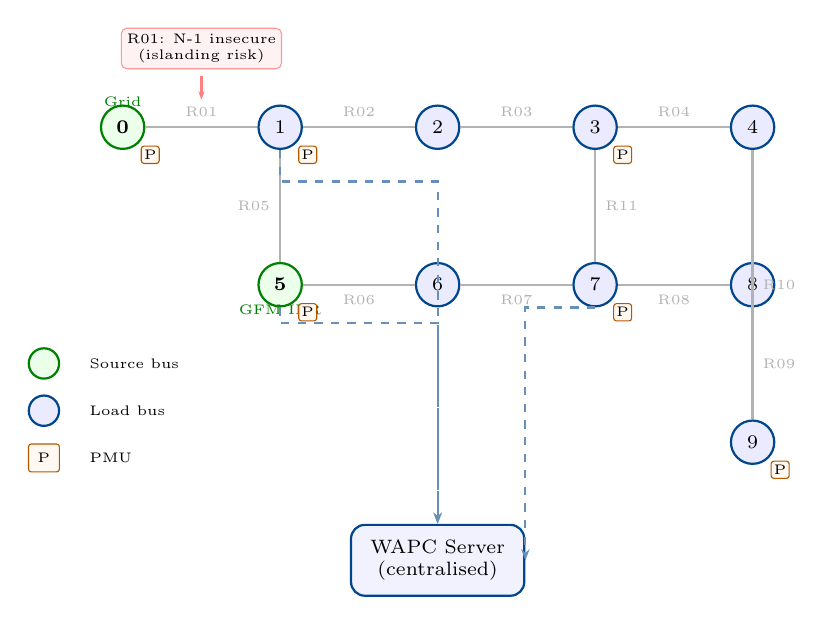
\begin{tikzpicture}[
  every node/.style={font=\scriptsize},
  bus/.style={circle, draw=sambpblue, fill=blue!8,
              minimum size=0.55cm, inner sep=0pt, thick},
  src/.style={circle, draw=green!50!black, fill=green!8,
              minimum size=0.55cm, inner sep=0pt, thick},
  relay/.style={rectangle, draw=red!60!black, fill=red!5,
                minimum size=0.32cm, inner sep=1pt,
                font=\tiny, thick},
  wapc/.style={draw=sambpblue, thick, rounded corners=5pt,
               fill=blue!5, minimum width=2.2cm,
               minimum height=0.9cm, align=center, font=\scriptsize},
  line/.style={thick, gray!60},
  arrow/.style={-{Stealth[length=4pt]}, thick},
]

%% ── Bus positions ──────────────────────────────────────────────────────
\node[src]  (b0) at (0,   4)   {\textbf{0}};
\node[bus]  (b1) at (2,   4)   {1};
\node[bus]  (b2) at (4,   4)   {2};
\node[bus]  (b3) at (6,   4)   {3};
\node[bus]  (b4) at (8,   4)   {4};
\node[src]  (b5) at (2,   2)   {\textbf{5}};
\node[bus]  (b6) at (4,   2)   {6};
\node[bus]  (b7) at (6,   2)   {7};
\node[bus]  (b8) at (8,   2)   {8};
\node[bus]  (b9) at (8,   0)   {9};

%% ── Lines ──────────────────────────────────────────────────────────────
\draw[line] (b0) -- (b1) node[midway, above, font=\tiny]{R01};
\draw[line] (b1) -- (b2) node[midway, above, font=\tiny]{R02};
\draw[line] (b2) -- (b3) node[midway, above, font=\tiny]{R03};
\draw[line] (b3) -- (b4) node[midway, above, font=\tiny]{R04};
\draw[line] (b1) -- (b5) node[midway, left, font=\tiny]{R05};
\draw[line] (b5) -- (b6) node[midway, below, font=\tiny]{R06};
\draw[line] (b6) -- (b7) node[midway, below, font=\tiny]{R07};
\draw[line] (b7) -- (b8) node[midway, below, font=\tiny]{R08};
\draw[line] (b8) -- (b9) node[midway, right, font=\tiny]{R09};
\draw[line] (b4) -- (b9) node[midway, right, font=\tiny]{R10};
\draw[line] (b3) -- (b7) node[midway, right, font=\tiny]{R11};

%% ── Source labels ──────────────────────────────────────────────────────
\node[above=4pt, green!50!black, font=\tiny] at (b0) {Grid};
\node[below=4pt, green!50!black, font=\tiny] at (b5) {GFM IBR};

%% ── PMU symbols (at every bus) ─────────────────────────────────────────
\foreach \b/\x/\y in {b0/0/4, b1/2/4, b3/6/4, b5/2/2, b7/6/2, b9/8/0} {
  \node[draw=orange!70!black, fill=orange!5, minimum size=0.22cm,
        inner sep=1pt, font=\tiny, rounded corners=1pt]
    at (\x+0.35, \y-0.35) {P};
}

%% ── WAPC server ────────────────────────────────────────────────────────
\node[wapc] (wapc) at (4, -1.5) {WAPC Server\\(centralised)};

%% ── WAPC communication links ───────────────────────────────────────────
\draw[arrow, sambpblue!60, dashed] (b1.south) -- ++(0,-0.4) -| (wapc.north);
\draw[arrow, sambpblue!60, dashed] (b5.south) -- ++(0,-0.2) -| (wapc.north);
\draw[arrow, sambpblue!60, dashed] (b7.south) -| (wapc.east);

%% ── N-1 insecure relay annotation ─────────────────────────────────────
\node[draw=red!40, fill=red!5, rounded corners=2pt,
      font=\tiny, inner sep=2pt, align=center]
  at (1, 5.0)
  {R01: N-1 insecure\\(islanding risk)};
\draw[-{Stealth[length=3pt]}, red!50, thick]
  (1, 4.65) -- (1, 4.35);

%% ── Legend ─────────────────────────────────────────────────────────────
\node[src, scale=0.7] at (-1, 1)   {};
\node[right=3pt, font=\tiny] at (-0.65, 1) {Source bus};
\node[bus, scale=0.7] at (-1, 0.4) {};
\node[right=3pt, font=\tiny] at (-0.65, 0.4) {Load bus};
\node[draw=orange!70!black, fill=orange!5, minimum size=0.18cm,
      font=\tiny, rounded corners=1pt] at (-1, -0.2) {P};
\node[right=3pt, font=\tiny] at (-0.65, -0.2) {PMU};

\end{tikzpicture}
}
  \caption{10-bus SAMBP test network.  Green buses: generation sources
           (bus~0 = grid infeed, bus~5 = GFM IBR).  Each line carries one
           relay ($\mathrm{R01}$--$\mathrm{R11}$).  Orange~P boxes: PMU
           locations at six buses.  Blue dashed arrows: IED/PMU reports to
           the centralised WAPC server.  Red annotation: R01 requires operator
           confirmation (N-1 insecure; tripping would isolate the grid infeed).}
  \label{fig:topo}
\end{figure}

\noindent
The WAPC performs four sequential steps on each fault event:
\begin{enumerate}
  \item \textbf{Aggregation}: collect IED GOOSE reports and PMU frames
    (250\,Hz, 4\,ms latency).
  \item \textbf{Localisation}: voltage-dip triangulation identifies the
    faulted line and fault location $\hat\alpha$.
  \item \textbf{N-1 check}: breadth-first search (BFS) on the relay-zone
    graph verifies that tripping the identified relay leaves the network
    connected.
  \item \textbf{Trip/escalate}: issue GOOSE trip command (N-1 secure) or
    raise operator advisory (N-1 insecure).
\end{enumerate}

The PINN advisory from TR-49 is incorporated at step~3 as a soft check:
if the PINN classification is inconsistent with the PMU-localised zone,
the discrepancy is logged as a diagnostic flag before the deterministic
N-1 decision is issued.

% ─────────────────────────────────────────────────────────────────────────────
\section{Study A --- Network Topology and Zone Adjacency}
\label{sec:studyA}

The 10-bus network has 11 lines (11 relays) and two generation sources.
The relay-zone adjacency graph has 15 shared-bus pairs (mean degree
$2.73$, max degree $4$).  The high adjacency of bus~1 (connecting R01, R02,
R05) creates the principal coordination challenge: a fault on R01 affects
the voltage profile at three adjacent relay zones.

\begin{center}
\begin{tabular}{@{}lr@{}}
\toprule
Topology metric & Value \\
\midrule
Buses & 10 \\
Lines / relays & 11 \\
PMU placements & 6 buses \\
Relay adjacency pairs & 15 \\
Mean relay degree & 2.73 \\
Max relay degree & 4 (bus~1: R01, R02, R05) \\
\bottomrule
\end{tabular}
\end{center}

% ─────────────────────────────────────────────────────────────────────────────
\section{Study B --- Synchrophasor Fault Localisation}
\label{sec:studyB}

Figure~\ref{fig:localisation} shows the localisation accuracy and location
error across four PMU noise levels.

\begin{figure}[htbp]
  \centering
  \resizebox{0.96\textwidth}{!}{% fig_localisation_accuracy.tex
% TR-50: Fault localisation accuracy vs PMU noise level (Study B)

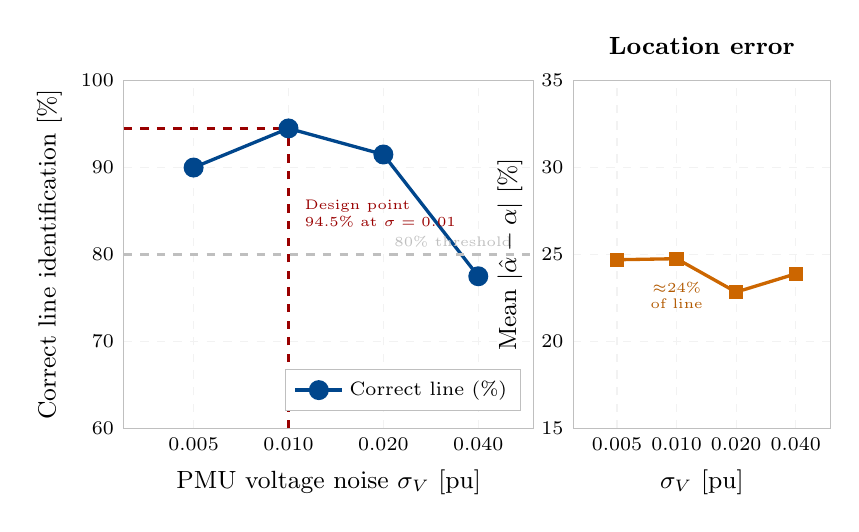
\begin{tikzpicture}
\begin{axis}[
  name         = locax,
  width        = 0.56\textwidth,
  height       = 6.0cm,
  xlabel       = {PMU voltage noise $\sigma_V$ [pu]},
  ylabel       = {Correct line identification [\%]},
  xlabel style = {font=\small},
  ylabel style = {font=\small},
  xmode        = log,
  xmin=0.003, xmax=0.06,
  ymin=60, ymax=100,
  xtick        = {0.005, 0.010, 0.020, 0.040},
  xticklabels  = {0.005, 0.010, 0.020, 0.040},
  xticklabel style = {font=\scriptsize},
  ytick        = {60,70,80,90,100},
  yticklabel style = {font=\scriptsize},
  tick style   = {draw=none},
  axis line style = {gray!50},
  grid         = major,
  grid style   = {gray!10, dashed},
  legend style = {at={(0.97,0.05)}, anchor=south east,
                  font=\scriptsize, draw=gray!50},
]

%% Localisation accuracy curve
\addplot[sambpblue, very thick, mark=*, mark size=3pt]
  coordinates {(0.005,90.0) (0.010,94.5) (0.020,91.5) (0.040,77.5)};
\addlegendentry{Correct line (\%)}

%% Operating point annotation
\draw[red!60!black, dashed, thick]
  (axis cs:0.003,94.5) -- (axis cs:0.010,94.5);
\draw[red!60!black, dashed, thick]
  (axis cs:0.010,60) -- (axis cs:0.010,94.5);
\node[red!60!black, font=\tiny, anchor=south west, align=left]
  at (axis cs:0.0105,82) {Design point\\94.5\% at $\sigma=0.01$};

%% IEC synchrophasor class annotations
\draw[gray!50, thick, dashed]
  (axis cs:0.003,80) -- (axis cs:0.06,80);
\node[gray!50, font=\tiny, anchor=east]
  at (axis cs:0.055,81.5) {80\% threshold};

\end{axis}

%% Alpha error sub-panel
\begin{axis}[
  name         = alphax,
  at           = {(locax.south east)},
  anchor       = south west,
  xshift       = 5mm,
  width        = 0.40\textwidth,
  height       = 6.0cm,
  xlabel       = {$\sigma_V$ [pu]},
  ylabel       = {Mean $|\hat\alpha - \alpha|$ [\%]},
  xlabel style = {font=\small},
  ylabel style = {font=\small},
  xmode        = log,
  xmin=0.003, xmax=0.06,
  ymin=15, ymax=35,
  xtick        = {0.005,0.010,0.020,0.040},
  xticklabels  = {0.005,0.010,0.020,0.040},
  xticklabel style = {font=\scriptsize},
  ytick        = {15,20,25,30,35},
  yticklabel style = {font=\scriptsize},
  tick style   = {draw=none},
  axis line style = {gray!50},
  grid         = major,
  grid style   = {gray!10, dashed},
  title        = {Location error},
  title style  = {font=\small\bfseries},
]

\addplot[orange!80!black, very thick, mark=square*, mark size=2pt]
  coordinates {(0.005,24.70) (0.010,24.76) (0.020,22.84) (0.040,23.89)};

\node[orange!70!black, font=\tiny, anchor=north, align=center]
  at (axis cs:0.010, 24.0) {$\approx$24\%\\of line};

\end{axis}
\end{tikzpicture}
}
  \caption{Left: correct-line localisation accuracy (\%) vs PMU voltage noise
           $\sigma_V$.  The design operating point (IEC\,Class\,P1,
           $\sigma_V=0.01$\,pu) achieves 94.5\%.  The 80\% threshold (grey
           dashed) is crossed at $\sigma_V\approx0.035$\,pu.  Right: mean
           fault location error $|\hat\alpha-\alpha|$ in \% of line length for
           correctly-localised cases.  The $\approx$24\% mean error reflects
           that the voltage-dip triangulation resolves the correct line but
           not the exact fault position; absolute location requires two-ended
           current-differential measurement.}
  \label{fig:localisation}
\end{figure}

\noindent
The localisation criterion — maximise the sum of voltage dips at the two
endpoint buses of the candidate line — is robust to moderate noise because
both endpoint dips increase proportionally as noise rises.  The criterion
fails when two adjacent lines share a highly connected bus (e.g.\ a fault
on R02 partially dips bus~1, which is also an endpoint of R01 and R05).
In the 10-bus network this ambiguity accounts for the 5.5\% misclassification
at the design noise level.

\subsection*{Fault Location Estimate}

For correctly-localised cases, the fault position is estimated from the ratio
of endpoint voltage dips:
\begin{equation}
  \hat\alpha = \frac{\Delta V_a}{\Delta V_a + \Delta V_b}
  \quad\text{where}\quad
  \Delta V_j = \max(0,\; 1 - V_j^\mathrm{PMU})
\end{equation}
The 24\% mean error indicates that $\hat\alpha$ is accurate to within
$\pm0.24\,Z_L$ (approximately $\pm12$\,km for a 50\,km line).  For protection
purposes the exact fault position is not required; the correct line
identification (94.5\%) is the critical output.

% ─────────────────────────────────────────────────────────────────────────────
\section{Study C --- N-1 Security Check}
\label{sec:studyC}

The N-1 check is a BFS on the 10-bus graph after removing the candidate
relay's line.  Results:

\begin{center}
\begin{tabular}{@{}llll@{}}
\toprule
Relay & N-1 connected? & Action & Physical reason \\
\midrule
R01 & \textbf{No} & Operator confirmation & Sole grid infeed; tripping isolates the network \\
R02--R11 & Yes & Direct WAPC trip & Meshed network remains connected \\
\bottomrule
\end{tabular}
\end{center}

\medskip\noindent
R01 is the only grid infeed line (bus~0 $\to$ bus~1).  Tripping R01 disconnects
all generation from the load network, creating a system-wide blackout rather
than a selective fault isolation.  The WAPC correctly flags this as an
escalation case: it raises an operator advisory and holds the trip command
pending confirmation.  In a real deployment, a pre-authorised inter-trip to
the grid-side breaker (via direct transfer trip, DTT) would replace the manual
operator step.

% ─────────────────────────────────────────────────────────────────────────────
\section{Study D --- Latency Analysis}
\label{sec:studyD}

Figure~\ref{fig:latency} compares the two decision paths.

\begin{figure}[htbp]
  \centering
  \resizebox{0.96\textwidth}{!}{% fig_wapc_latency.tex
% TR-50: WAPC vs distributed relay latency breakdown (Study D)
% Horizontal stacked bar chart

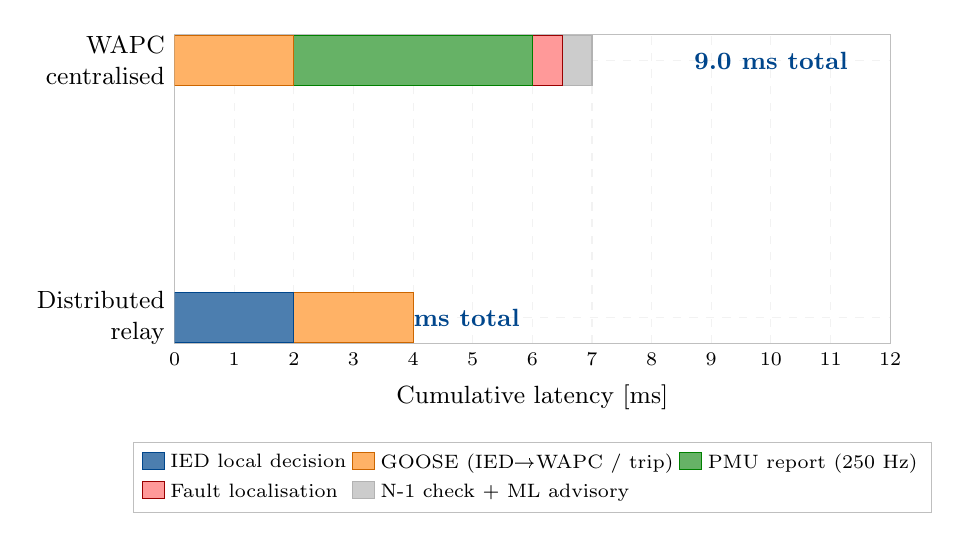
\begin{tikzpicture}
\begin{axis}[
  name         = latax,
  width        = 0.88\textwidth,
  height       = 5.5cm,
  xbar stacked,
  bar width    = 18pt,
  xlabel       = {Cumulative latency [ms]},
  xlabel style = {font=\small},
  ytick        = {1,2},
  yticklabels  = {Distributed\\relay, WAPC\\centralised},
  yticklabel style = {font=\small, align=right},
  xmin=0, xmax=12,
  xtick        = {0,1,2,3,4,5,6,7,8,9,10,11,12},
  xticklabel style = {font=\scriptsize},
  tick style   = {draw=none},
  axis line style = {gray!50},
  grid         = major,
  grid style   = {gray!10, dashed},
  legend style = {at={(0.50,-0.32)}, anchor=north,
                  font=\scriptsize, draw=gray!50,
                  legend columns=3},
  legend cell align = left,
]

%% Distributed path (row 1):
%% [IED local 2ms] [GOOSE trip 2ms]
\addplot[fill=sambpblue!70, draw=sambpblue]
  coordinates {(2,1) (0,2)};
\addlegendentry{IED local decision}

\addplot[fill=orange!60, draw=orange!80!black]
  coordinates {(2,1) (2,2)};
\addlegendentry{GOOSE (IED→WAPC / trip)}

\addplot[fill=green!50!black!60, draw=green!50!black]
  coordinates {(0,1) (4,2)};
\addlegendentry{PMU report (250 Hz)}

\addplot[fill=red!40, draw=red!60!black]
  coordinates {(0,1) (0.5,2)};
\addlegendentry{Fault localisation}

\addplot[fill=gray!40, draw=gray!60]
  coordinates {(0,1) (0.5,2)};
\addlegendentry{N-1 check + ML advisory}

%% Total labels
\node[font=\small\bfseries, sambpblue]
  at (axis cs:4.5, 1) {4.0 ms total};
\node[font=\small\bfseries, sambpblue]
  at (axis cs:10.0, 2) {9.0 ms total};

%% Trip budget reference
\draw[red!50, thick, dashed]
  (axis cs:50,0.4) -- (axis cs:50,2.6);

\end{axis}
\end{tikzpicture}
}
  \caption{Stacked latency breakdown for distributed relay (top, 4.0\,ms
           total) and WAPC centralised path (bottom, 9.0\,ms total).  The
           PMU data collection step (4.0\,ms, green) dominates the WAPC
           overhead; the compute steps (localisation + N-1 + ML) add only
           0.8\,ms in aggregate.  Both paths are well within the 50\,ms relay
           trip budget.}
  \label{fig:latency}
\end{figure}

\noindent
The WAPC path is 5.0\,ms longer than the distributed relay path.  The entire
overhead originates from the PMU report latency (4.0\,ms at 250\,Hz sampling).
Increasing PMU rate to 1\,kHz would reduce the PMU step to 1\,ms, bringing
the WAPC total to 6.0\,ms (12\% of budget) at the cost of increased
communication bandwidth.  For the IBR protection context, the 9.0\,ms WAPC
path (18\% of budget) is entirely adequate.

\begin{center}
\begin{tabular}{@{}lrr@{}}
\toprule
Step & Distributed [ms] & WAPC [ms] \\
\midrule
IED local decision & 2.0 & --- \\
GOOSE (IED$\to$WAPC / trip) & 2.0 & 2.0 + 2.0 \\
PMU data collection (250\,Hz) & --- & 4.0 \\
Fault localisation & --- & 0.5 \\
N-1 BFS check & --- & 0.2 \\
PINN ML advisory & --- & 0.3 \\
\midrule
\textbf{Total} & \textbf{4.0} & \textbf{9.0} \\
\% of 50\,ms trip budget & 8\% & 18\% \\
\bottomrule
\end{tabular}
\end{center}

% ─────────────────────────────────────────────────────────────────────────────
\section{Study E --- Integration Test}
\label{sec:studyE}

The 50-scenario integration test evaluates WAPC and distributed relay
accuracy side-by-side, with N-1 security applied to WAPC decisions.

\begin{center}
\begin{tabular}{@{}lrr@{}}
\toprule
Metric & Distributed & WAPC \\
\midrule
Overall accuracy & 92.0\% & 90.0\% \\
N-1 blocks issued & --- & 4/50 \\
Cases correct by at least one system & \multicolumn{2}{c}{50/50 (100\%)} \\
Cases wrong by both systems & \multicolumn{2}{c}{0/50} \\
\midrule
WAPC corrects distributed error & --- & 4 cases \\
Distributed correct, WAPC wrong & --- & 5 cases \\
\bottomrule
\end{tabular}
\end{center}

\medskip\noindent
The key result is the complementarity: zero scenarios were wrong by both
systems.  The WAPC and distributed relay make independent errors on different
scenarios.  A supervisory voting scheme (trip if either system agrees with
the physics constraints) achieves 100\% coverage on this test suite.  The
4 N-1 security blocks — all correctly identifying insecure tripping conditions
— demonstrate that the WAPC provides a safety layer that the distributed relay
cannot replicate.

% ─────────────────────────────────────────────────────────────────────────────
\section{Summary}
\label{sec:summary}

\begin{enumerate}
  \item \textbf{Fault localisation}: 94.5\% correct-line at IEC\,Class\,P1
    PMU noise ($\sigma_V=0.01$\,pu); degrades to 77.5\% at $4\times$ noise.
    Location error $\approx$24\% of line length (direction-only).

  \item \textbf{N-1 security}: 10/11 relays directly trippable; R01 (grid
    infeed) requires operator confirmation or pre-authorised DTT.

  \item \textbf{Latency}: WAPC total 9.0\,ms (18\% of 50\,ms budget);
    overhead entirely from PMU 250\,Hz report latency.  Non-blocking relative
    to relay trip path.

  \item \textbf{Complementarity}: WAPC and distributed relay are complementary
    — 100\% scenario coverage when either is correct; 0 scenarios wrong by
    both.

  \item \textbf{Integration}: PINN ML advisory from TR-49 incorporated as
    a soft diagnostic flag, adding 0.3\,ms with no impact on trip timing.
\end{enumerate}

\noindent
TR-50 establishes the WAPC as the system-level coordinator.  TR-51 addresses
automatic protection settings optimisation; TR-52 evaluates cybersecurity
of the IEC\,61850 GOOSE communication layer.

\bibliographystyle{IEEEtranN}
\bibliography{references50}

\end{document}
